\documentclass[10pt]{beamer}

\usepackage[T2A]{fontenc}
\usepackage[utf8]{inputenc}
\usepackage[russian,english]{babel}

\usefonttheme[onlymath]{serif}

\usetheme[progressbar=frametitle]{metropolis}
\usepackage{appendixnumberbeamer}

\usepackage{booktabs}
\usepackage[scale=2]{ccicons}

\usepackage{pgfplots}
\usepgfplotslibrary{dateplot}

\usepackage{xspace}
\newcommand{\themename}{\textbf{\textsc{metropolis}}\xspace}
\newcommand{\TODO}[1]{\textbf{\textcolor{red}{TODO: #1}}}

\date{}
\author{Екатерина Тузова}


\title{Лекция 2}
\subtitle{Метрические классификаторы}
\usepackage{subfig}

\begin{document}

\maketitle

\section{Разбор летучки}

\section{Мотивирующий пример}

{\setbeamertemplate{frame footer}{\href{https://www.kaggle.com/abcsds/pokemon}{Pokemon with stats (https://www.kaggle.com/abcsds/pokemon)}}
\begin{frame}{Мотивирующий пример}
	\begin{figure}
	    \centering
	    \subfloat{{
\includegraphics[width=2cm]{images/Bulbasaur} }}
	    \qquad
	    \subfloat{{
\includegraphics[width=2cm]{images/Mewtwo} }}
    	    \qquad
    	    \subfloat{{
\includegraphics[width=2cm]{images/Volcanion} }}
    	    \qquad
    	    \subfloat{{
\includegraphics[width=2cm]{images/Ekans} }}
    	    \qquad
    	    \subfloat{{
\includegraphics[width=2cm]{images/Nidorina} }}
	    \qquad 
    	    \subfloat{{
\includegraphics[width=2cm]{images/Rattata} }}
	    \qquad
    	    \subfloat{{
\includegraphics[width=2cm]{images/Sandshrew} }}
	    \qquad
    	    \subfloat{{
\includegraphics[width=2cm]{images/Articuno} }}    	        	    
	\end{figure}
\end{frame}
}

\begin{frame}{Датасет}
    \centering
	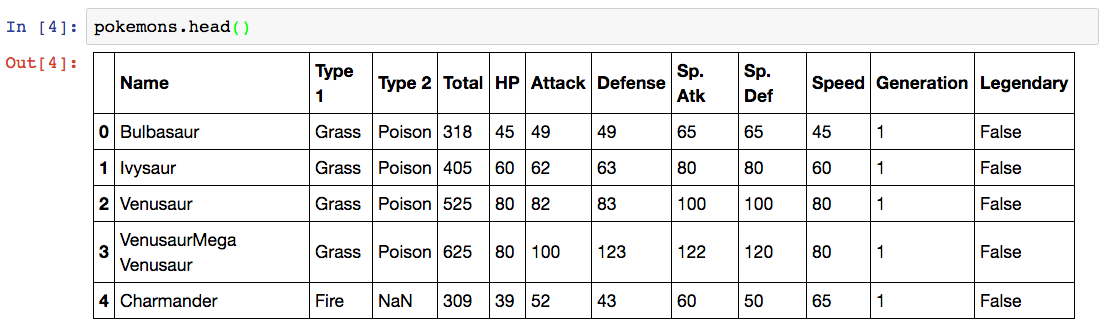
\includegraphics[width=\textwidth]{images/pokemons}
\end{frame}

\section{Какие признаки есть в датасете?}

\begin{frame}
	${f: X \rightarrow D_f}$
	\begin{enumerate} [-]
	  \item Бинарные (${D_f = \left\{ 0, 1 \right\} }$)
	  \item Номинальные (${D_f}$ -- конечное множество)
	  \item Порядковые (${D_f}$ -- конечное упорядоченное множество)
	  \item Количественные (${D_f = \mathbb{R} }$)
	\end{enumerate}
\end{frame}

\begin{frame}{Признаки}
	\begin{enumerate} [-]	
		\item Бинарные (Legendary)
		\item Номинальные (Type 1, Type 2)
		\item Порядковые (Generation)
		\item Количественные (Attack, Defense, ...)
	\end{enumerate}
\end{frame}

\begin{frame}{Легендарность}
\alert{Легендарный покемон} это чрезвычайно редкий и зачастую очень могущественных покемон, о нем слагаются мифы и легенды в мире покемонов.
\end{frame}

\begin{frame}{Легендарность}
	\begin{figure}
	    \centering
	    \subfloat{{
\includegraphics[width=2cm]{images/Bulbasaur} }}
	    \qquad
	    \subfloat{\frame{
\includegraphics[width=2cm]{images/Mewtwo} }}
    	    \qquad
    	    \subfloat{\frame{
\includegraphics[width=2cm]{images/Volcanion} }}
    	    \qquad
    	    \subfloat{{
\includegraphics[width=2cm]{images/Ekans} }}
    	    \qquad
    	    \subfloat{{
\includegraphics[width=2cm]{images/Nidorina} }}
	    \qquad 
    	    \subfloat{{
\includegraphics[width=2cm]{images/Rattata} }}
	    \qquad
    	    \subfloat{{
\includegraphics[width=2cm]{images/Sandshrew} }}
	    \qquad
    	    \subfloat{\frame{
\includegraphics[width=2cm]{images/Articuno} }}    	        	    
	\end{figure}
\end{frame}

\begin{frame}{Распределение}
    \centering
	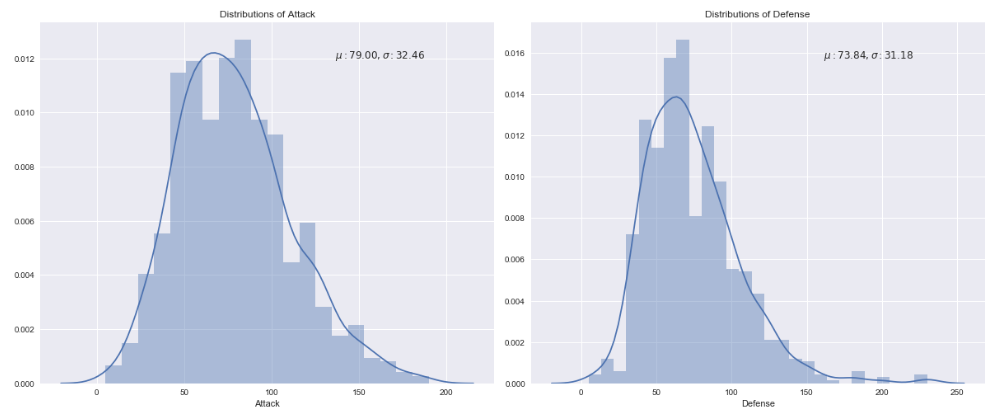
\includegraphics[width=\textwidth]{images/attack_defense}
	
	Number of Pokemons = 800
\end{frame}

{\setbeamertemplate{frame footer}{\href{https://github.com/ktisha/ML2017/tree/master/notebooks}{Репозиторий с материалами (https://github.com/ktisha/ML2017))}}
\begin{frame}{Типы покемонов}
    \centering
	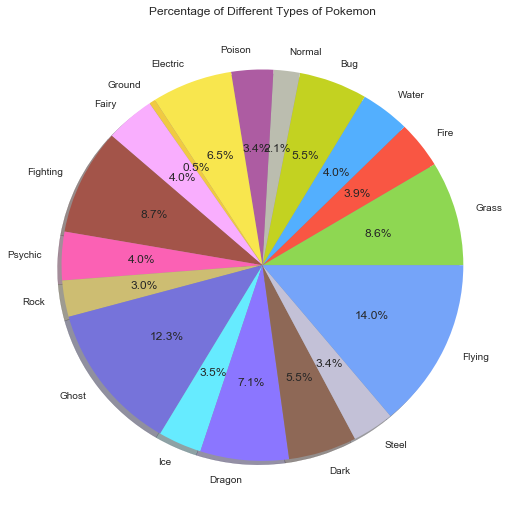
\includegraphics[width=\linewidth,height=0.8 \textheight,keepaspectratio]{images/pokemons_by_type}
\end{frame}
}

\begin{frame}{Задача классификации}
	$X$ - множество объектов \\
	$Y$ - множество классов \\
	Обучающая выборка: ${X^l = (x_i, y_i)_{i=1}^l}$ \\ 
	\bigbreak
	\bigbreak
	\alert{Задача}: Построить алгоритм ${a \colon X \rightarrow Y}$, способный классифицировать произвольный объект ${x \in X}$.
\end{frame}

\begin{frame}{Задача классификации в нашем контексте}
	$X$ - покемоны \\
	$Y$ - легендарность \\
	Обучающая выборка: ${X^l = (x_i, y_i)_{i=1}^l}$ \\ 
	$l = 800$ покемонов в выборке\\
	\bigbreak
	\alert{Задача}: Построить алгоритм ${a \colon X \rightarrow Y}$, способный определить, является ли покемон легендарным.
\end{frame}

\section{Гипотеза компактности}

\begin{frame}{Гипотеза компактности}
    \centering
 	Схожие объекты, как правило, лежат в одном классе.\\
\end{frame}

\begin{frame}{Пример}
    \centering
	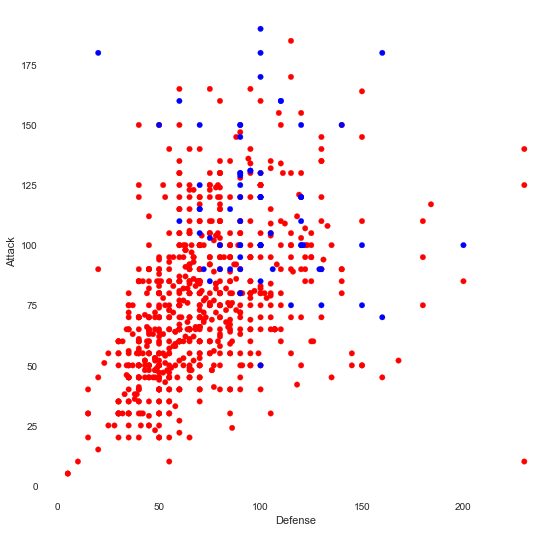
\includegraphics[width=\linewidth,height=0.8 \textheight,keepaspectratio]{images/attack_vs_defense}
\end{frame}

\begin{frame}{Гипотеза компактности}
	Схожие объекты, как правило, лежат в одном классе.\\
	\bigbreak
	Как определить \alert{схожесть} объектов?\\
\end{frame}

\begin{frame}{Гипотеза компактности}
	Схожие объекты, как правило, лежат в одном классе.\\
	\bigbreak
	\alert{Схожесть} $=$ Функция расстояния:\\
	${\rho: X \times X \rightarrow [0, \infty) }$
\end{frame}

\section{Функции расстояния}

{\setbeamertemplate{frame footer}{Euclidean distance (metric)}
\begin{frame}{Евклидово расстояние}
	${\rho (u, v) = \sqrt{\sum\limits_{j=1}^n |u^j - v^j|^2}}$, \hspace{5mm} ${u, v \in X^{l}}$\\
	\bigbreak
	
	Признаковые описания объектов:\\
	${u = \left\{ u^1, u^2, ..., u^n \right\}}$ \\
	${v = \left\{v^1, v^2, ..., v^n \right\} }$ 
\end{frame}
}

{\setbeamertemplate{frame footer}{Манхэттенское расстояние, Taxicab distance}
\begin{frame}{Расстояние городских кварталов}
	${\rho (u, v) = \sum\limits_{j=1}^n |u^j - v^j|}$, \hspace{5mm} ${u, v \in X^{l}}$\\
	\bigbreak
	
	Признаковые описания объектов:\\
	${u = \left\{ u^1, u^2, ..., u^n \right\}}$ \\
	${v = \left\{v^1, v^2, ..., v^n \right\} }$ 
\end{frame}
}

{\setbeamertemplate{frame footer}{Minkowski distance}
\begin{frame}{Расстояние Минковского}
	Обобщение евклидова расстояния и расстояния городских кварталов
	\bigbreak
	${\rho (u, v) = (\sum\limits_{j=1}^n |u^j - v^j|^q)^{1/q}}$, \hspace{5mm} ${u, v \in X^{l}}$\\
	\bigbreak
	
	Признаковые описания объектов:\\
	${u = \left\{ u^1, u^2, ..., u^n \right\}}$ \\
	${v = \left\{v^1, v^2, ..., v^n \right\} }$ 
\end{frame}
}

{\setbeamertemplate{frame footer}{Редакционное расстояние, дистанция редактирования, Edit distance }
\begin{frame}{Расстояние Левенштейна}
	Минимальное количество операций вставки одного символа, удаления одного символа и замены одного символа на другой, необходимых для превращения одной строки в другую.
\end{frame}
}

\section{Метрический классификатор}

\begin{frame}{Обобщенный метрический классификатор}
	$u \in X$ - произвольный объект, который собираемся классифицировать.\\
	\bigbreak
	Отсортируем объекты $x_1, x_2, ..., x_l$ относительно $u$:
	${\rho(u, x_1) \leq \rho(u, x_2) \leq \dots \leq \rho(u, x_l)}$\\
	\bigbreak
	${x_i}$ -- $i$-й сосед объекта $u$\\
	${y_i}$ -- класс $i$-го соседа объекта $u$
\end{frame}

\begin{frame}{Метрический алгоритм классификации}
	${a(u, X^l) = \arg\max\limits_{y \in Y} \underbrace{\sum\limits_{y_i = y} w(i, u)}_{\Gamma_y(u)} }$\\
	\vspace{5mm}
	$w(i, u)$ - вес $i$-го соседа $u$, неотрицателен\\
	$\Gamma_y(u)$ - оценка близости объекта $u$ к классу ${y}$
\end{frame}

\begin{frame}{Метод ближайшего соседа}
	Объект относится к тому классу, к которому относится ближайший в выборке.\\
	${w(i, u) = [i=1]}$\\
\end{frame}

\begin{frame}{Метод ближайшего соседа}
	Объект относится к тому классу, к которому относится ближайший в выборке.\\
	${w(i, u) = [i=1]}$\\
	\bigbreak
	\begin{itemize} [<+- | alert@+>]
		\item[+] Простота
		\item[+] Интерпретируемость решения
	  \bigbreak
		\item[--	] Неустойчивость к шуму
		\item[--	] Отсутствие настраиваемых параметров
		\item[--	] Низкое качество классификации
		\item[--	] Необходимость хранить всю выборку целиком		
	\end{itemize}
\end{frame}

\begin{frame}{Пример}
	\begin{frame}{Пример}
    \centering
	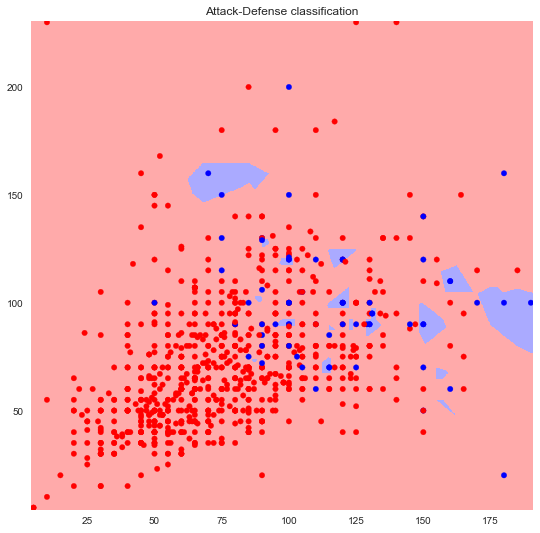
\includegraphics[width=\linewidth,height=0.8 \textheight,keepaspectratio]{images/attack_vs_defense_fail}
\end{frame}

\end{frame}

\begin{frame}{Метод k ближайших соседей}
	${w(i, u) = [i \leq k]}$\\
	\bigbreak
	\begin{itemize} [<+- | alert@+>]
		\item[+] Менее чувствителен к шуму
		\item[+] Появляется настраиваемый параметр k
	  \bigbreak
	  \item[--] Неоднозначность классификации при ${\Gamma_y(u) = \Gamma_s(u), y \neq s}$
	\end{itemize}
\end{frame}

\section{Подбор параметров}

\begin{frame}{Как выбрать $k$}
	Функционал скользящего контроля (leave-one-out):\\
	${LOO(k, X^l) = \sum\limits_{i=1}^l [a(x_i; X^l \backslash \left\{x_i\right\}, k) \neq y] \rightarrow \min\limits_k}$\\
\end{frame}

\begin{frame}{Вопрос}
	Правда ли нужно выбрасывать один объект?
\end{frame}

\begin{frame}{Ответ}
	\TODO{картинка с пояснением почему нужно. переобучение}
\end{frame}

\begin{frame}{Метод $k$ взвешенных соседей}
	${w(i,u) = [i \leq k] * w_i}$, где $w_i$ это вес, зависящий только от номера соседа\\
	\bigbreak
	Возможные эвристики:\\
	\begin{itemize} [<+- | alert@+>]
	\item[--] ${w_i = \frac{k+1-i}{k}}$ -- линейное убывающие веса\\ % почему плохо?
	\item[--] ${w_i = q^i}$ -- экспоненциально убывающие веса\\
	\end{itemize}
\end{frame}

\begin{frame}{Вопрос}
	Как более обоснованно задать веса?\\
\end{frame}

\begin{frame}{Ядерная оценка плотности}
	\textbf{Метод окна Парзена}\\
	${w_i = K(\frac{\rho(u, x^i)}{h})}$\\
	$K(r)$ -- ядро, невозрастающее, положительное на ${[0, 1]}$\\
\end{frame}

\begin{frame}{Ядерная оценка плотности}
	\textbf{Метод окна Парзена}\\
	${w_i = K(\frac{\rho(u, x^i)}{h})}$\\
	$K(r)$ -- ядро, невозрастающее, положительное на ${[0, 1]}$\\
  \bigbreak
	Фиксированной ширины:\\
	${a(u, X^l, h, K) = \arg\max\limits_{y \in Y} \sum\limits_{i=1}^l [y^i = y] K(\frac{\rho(u, x^i)}{h})}$ \hspace{5mm} $h$ -- ширина окна\\
\end{frame}

\begin{frame}{Ядерная оценка плотности}
	\textbf{Метод окна Парзена}\\
	${w_i = K(\frac{\rho(u, x^i)}{h})}$\\
	$K(r)$ -- ядро, невозрастающее, положительное на ${[0, 1]}$\\
  \bigbreak
	Фиксированной ширины:\\
	${a(u, X^l, h, K) = \arg\max\limits_{y \in Y} \sum\limits_{i=1}^l [y^i = y] K(\frac{\rho(u, x^i)}{h})}$\\
	$h$ -- ширина окна\\
  \bigbreak
	Переменной ширины:\\
	${a(u, X^l, k, K) = \arg\max\limits_{y \in Y} \sum\limits_{i=1}^l [y^i = y] K(\frac{\rho(u, x^i)}{\rho(u, x^{k+1})})}$
\end{frame}

\begin{frame}{Более наглядно}
  \TODO{картинка с пояснением}
\end{frame}

\section{Выбор метрики}
% Какие метрики вам известны?\\
% Как выбрать подходящую? 
% http://arxiv.org/pdf/1306.6709v4.pdf

\begin{frame}{Выбор метрики. MMC}
	\alert{Идея}: Максимизировать сумму расстояний между объектами разных классов
	при этом сохраняя сумму расстояний между объектами одного класса небольшой.\\
	\bigbreak
	$${\max \sum\limits_{x_i, x_j \in D} \rho(x_i, x_j) }$$\\
	\bigbreak
	$${\sum\limits_{x_i, x_j \in S} \rho^2(x_i, x_j) \leq 1 }$$
\end{frame}

\begin{frame}{Проклятие размерности}
	Если используемая метрика ${\rho(u, x^i)}$ основана на суммировании различий по всем признакам, а число признаков очень велико,
	то все точки выборки могут оказаться практически одинаково далеки друг от друга.\\
\end{frame}

\begin{frame}{Пример}
	Набор признаков объекта генерируется подбрасыванием честной монетки $n$ раз. Соответственно
	каждый объект описывается вектором $[0, 1]^n$. При таких условиях все объекты будут равноудалены.
\end{frame}

\section{Предобработка}

\begin{frame}{Предобработка данных}
	Что делать если разные шкалы признаков?
\end{frame}

\begin{frame}{Предобработка данных}
	Все признаки должны быть представлены \alert{в одном масштабе}. \\
	В противном случае признак с наибольшими числовыми значениями будет доминировать в метрике.
\end{frame}


\begin{frame}{Жадное добавление признаков}
	\begin{itemize} [<+- | alert@+>]
		\item[--] ${\rho_j(u, x_i) = \vert u^j - x_i^j \vert}$ -- расстояние по j-му признаку\\
		          $LOO(j) \rightarrow \min$\\
		\item[--] Добавляем признак и строим $\rho'$\\
							${\rho'(u, x_i) = \rho(u, x_i) + w_j\rho_j(u, x_i)}$\\
							$LOO(j, w_j) \rightarrow \min$\\
		\item[--] Замена признака:\\
            		${\rho'(u, x_i) = \rho(u, x_i) - w_k\rho_k(u, x_i) + w_j\rho_j(u, x_i)}$\\
		\item[--] Добавляем признаки, пока LOO не увеличивается
	\end{itemize}
\end{frame}

\begin{frame}{Сверхбольшие выборки}
	\begin{itemize} [<+- | alert@+>]
		\item[--] Проблема хранения
		\item[--] Проблема быстрого поиска ближайших соседей
	\end{itemize}
\end{frame}

\begin{frame}{Отступ}
	Отступ показывает степень "типичности объекта".\\
	\bigbreak
	Отступом объекта ${x_i \in X^l}$ относительно классификатора $a$ называется величина\\
	${M(x_i) = \Gamma_{y_i}(x_i) - \max\limits_{y \in Y\backslash y_i} \Gamma_y(x_i)}$
\end{frame}

\begin{frame}{Типы объектов}
	\begin{enumerate}
		\item Эталонные
		\item Неинформативные
		\item Пограничные	
		\item Ошибочные	
		\item Шумовые	
	\end{enumerate}
\end{frame}

\begin{frame}{Типы объектов}
  \TODO{картинка с примером}
\end{frame}


\begin{frame}{Отбор эталонных объектов}
	\alert{Задача}:\\
	Ыыбрать оптимальное подмножество эталонов $\Omega\subseteq X^l$\\ 
  \bigbreak
	Классификатор будет иметь вид:\\
	${a(u, \Omega) = \arg\max\limits_{y \in Y} \sum\limits_{x_i \in \Omega} [y_u^i = y]w(i, u) }$\\
\end{frame}

\begin{frame}{Алгоритм STOLP}
	\begin{enumerate}
		\item Исключить выбросы и пограничные объекты
		\item Найти по одному эталону в каждом классе
		\item Добавлять эталоны, пока есть отрицательные отступы	
	\end{enumerate}
\end{frame}

\begin{frame}{Алгоритм STOLP}
	\begin{itemize} [<+- | alert@+>]
	\item[+] Сокращается число хранимых объектов
	\item[+] Сокращается время классификации
	\item[+] Объекты разделяются по величине отступа
	\bigbreak
	\item[--] Выбор параметра для определения выбросов
	\item[--] Не высокая эффективность
	\end{itemize}
\end{frame}

\section{Быстрый поиск ближайших соседей}

\begin{frame}{Быстрый поиск ближайших соседей}
	\begin{itemize}
		\item[--] граф ближайших соседей
		\item[--] k-d дерево
		\item[--] хеширование (LSH)
	\end{itemize}
\end{frame}

\begin{frame}[standout]
  Вопросы?
\end{frame}

\appendix


%\begin{frame}\frametitle{Что происходит сейчас в области knn}
	%A Ranking-based KNN Approach for Multi-Label Classification 2012
	% http://jmlr.org/proceedings/papers/v25/chiang12/chiang12.pdf
	
	%Fast Approximate kNN Graph Construction for High Dimensional
	%Data via Recursive Lanczos Bisection 2009
	%http://www.jmlr.org/papers/volume10/chen09b/chen09b.pdf
	
	%mahalanobis Distance Metric Learning for Large Margin
	%Nearest Neighbor Classification 2009
	%http://www.jmlr.org/papers/volume10/weinberger09a/weinberger09a.pdf
%\end{frame}

\begin{frame}\frametitle{Доп. ресурсы}
	\href{http://www.machinelearning.ru}{http://www.machinelearning.ru}\\
	\bigbreak
	\href{http://www.machinelearning.ru/wiki/images/6/6d/Voron-ML-1.pdf}{Пособие}
\end{frame}


\begin{frame}\frametitle{На следующей лекции}
	\begin{itemize}
		\item[--] Кластеризация.  K-means.
		\item[--] Цели кластеризации.
		\item[--] Типы кластерных структур.
		\item[--] Функционал качества кластеризации
		\item[--] К-средних
		\item[--] Иерархическая кластеризация.
	\end{itemize}
\end{frame}

\end{document}

              
